%% ---------------------------------------------------------------------
\section{Validation and characterisation}
\label{sec:validation}

\subsection{Scope and evidence levels}

\Cref{tab:evidence} shows where each result comes from. Items marked \emph{logged}
come with data in the repository, and their figures can be regenerated from
\code{report/scripts/}. Items marked \emph{dev.\ notes} are measurements we took during
development without keeping the raw data. We tested the real vehicle in a \SI{7}{\minute} hover over grass, measured against ground marks, and
in an autonomous square-path flight with obstacle avoidance (\cref{sec:val-hwdemo}).
Simulation flights, with Gazebo ground truth, are analysed in \cref{sec:val-simlogs}.

\begin{table}[H]
\centering\small
\caption{Validation evidence and its provenance.}
\label{tab:evidence}
\begin{tabularx}{\textwidth}{p{4.6cm} p{2.0cm} L}
\toprule
\textbf{Item} & \textbf{Source} & \textbf{Basis} \\
\midrule
Unit tests of segmentation logic & logged & 17 tests executed, \cref{sec:val-tests} \\
Bench sensor characterisation & logged & 25\,s autopilot log, \code{report/data/bench_telemetry_2026-11-15.csv} \\
ZUPT detector evaluation & logged & same log, bridge's parameters \\
IMU dead-reckoning drift & logged & same log, strapdown integration \\
Segmentation timing & logged & 100 frames $\times$ 3 configurations on RTX~4050 \\
Link-latency reductions & dev.\ notes & \code{docs/REFERENCE.md}, single-host measurement \\
Segmentation latency on drone feed & dev.\ notes & launch-file comment, \code{docs/REFERENCE.md} \\
Topic rates on the real vehicle & dev.\ notes & \code{docs/QUICKSTART.md} \\
LiDAR revolution rate, flag rate & dev.\ notes & source comment, \code{lidar_udp_streamer.py} \\
Real-vehicle hover drift & logged & \SI{7}{\minute} \code{GUIDED} hover at \SI{2.5}{\metre} over grass, ground marks \\
Autonomous square path + avoidance & logged & video (\cref{fig:hwdemo}) \\
Simulation behaviour & dev.\ notes & qualitative, \code{docs/SIMULATION.md}, video (\cref{fig:sim}) \\
Simulation flight metrics & logged & 26 PX4 SITL logs with Gazebo truth, \cref{sec:val-simlogs} \\
\bottomrule
\end{tabularx}
\end{table}

\subsection{Software unit tests}
\label{sec:val-tests}

The perception package contains 17 \code{pytest} cases for the ROS-independent fusion
and rasterisation logic. They check mask IoU, box expansion and clipping, acceptance of
a good SAM mask, fallback on a low SAM score, fallback on SAM--YOLO disagreement,
clipping of leaked masks, rejection of empty masks, selective refinement, the
detect-only model path, the no-SAM path, overlap ordering in rasterisation, and
SAM-family detection. All 17 passed on the benchmark host (\code{17 passed in
0.10s}). The ROS packages additionally carry the standard \code{flake8},
\code{pep257} and copyright tests.

\subsection{Bench characterisation of the autopilot sensors}
\label{sec:val-bench}

\paragraph{Protocol} The vehicle stood on a bench, disarmed, with no flight battery
connected (reported battery voltage \SI{0.19}{\volt}) and no GNSS fix
(0 satellites, fix type 0). Telemetry streamed from the Pi was logged on the laptop by
\code{plotjuggler_bridge.py} on 2026-11-15, for \SI{24.93}{\second} (243 samples).
The log predates the \SI{30}{\hertz} telemetry change, so the median rate was
\SI{9.91}{\hertz} (spacing $\SI{103.0}{}\pm\SI{17.0}{\milli\second}$, longest gap
\SI{302.6}{\milli\second}). The vehicle was pitched \SI{12.96}{\degree}, and the
disturbances near \SI{5}{\second} and \SIrange{13}{16}{\second} are unannotated.

\begin{figure}[t]
\centering
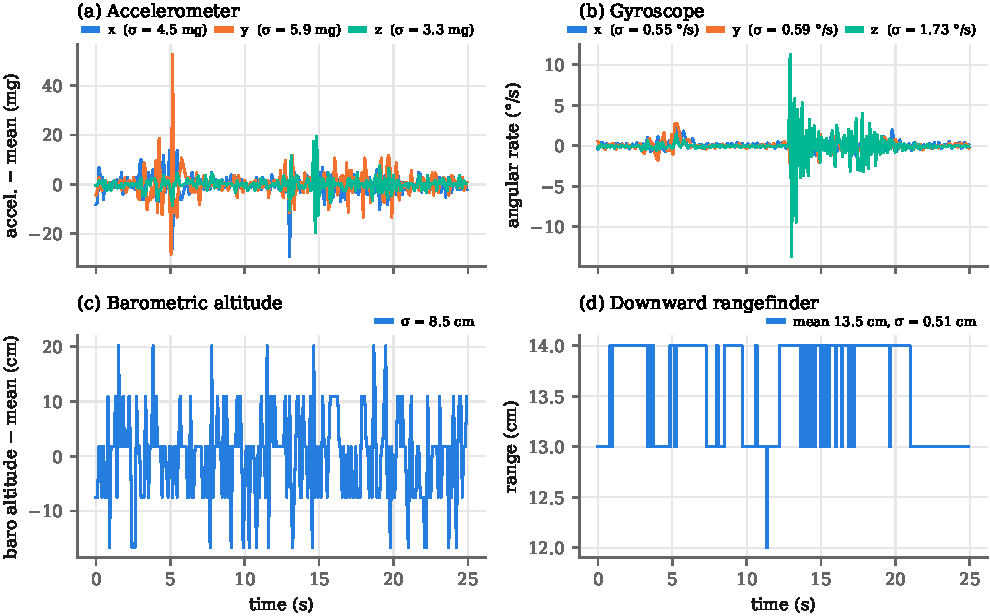
\includegraphics[width=\textwidth]{bench_sensor_noise.pdf}
\caption{Stationary bench log, vehicle disarmed. (a) Accelerometer deviation from the
mean; (b) gyroscope rate; (c) altitude computed from static pressure with
\cref{eq:baro}; (d) downward rangefinder. A transient disturbance is visible near
\SI{13}{\second}, mainly about the yaw axis.}
\label{fig:bench}
\end{figure}

\begin{table}[H]
\centering\small
\caption{Sensor statistics from the bench log (\cref{fig:bench}). $\sigma$ is the
standard deviation over the whole log, including the disturbances.}
\label{tab:bench}
\begin{tabular}{l S[table-format=4.1] S[table-format=1.2] l}
\toprule
\textbf{Channel} & {\textbf{Mean}} & {$\bm{\sigma}$} & \textbf{Remark} \\
\midrule
Accel $x$ (\si{\milli\gacc}) & 199.1 & 4.47 & pitch $\approx$\SI{13}{\degree} projects gravity \\
Accel $y$ (\si{\milli\gacc}) & 14.3 & 5.93 & \\
Accel $z$ (\si{\milli\gacc}) & -983.6 & 3.29 & $\lVert\mathbf{f}\rVert = 1003.6\pm\SI{2.9}{\milli\gacc}$ \\
Gyro $x$ (\si{\degree\per\second}) & 0.096 & 0.55 & \\
Gyro $y$ (\si{\degree\per\second}) & 0.030 & 0.59 & \\
Gyro $z$ (\si{\degree\per\second}) & -0.053 & 1.73 & inflated by the yaw transient \\
Static pressure (\si{\hecto\pascal}) & 895.01 & 0.0092 & resolution \SI{0.01}{\hecto\pascal} \\
Baro altitude (\si{\centi\metre}) & {--} & 8.46 & peak-to-peak \SI{36.8}{\centi\metre} \\
Rangefinder (\si{\centi\metre}) & 13.55 & 0.51 & \SI{1}{\centi\metre} quantisation \\
\bottomrule
\end{tabular}
\end{table}

\paragraph{Findings} $\sigma\lVert\mathbf{f}\rVert=\SI{2.9}{\milli\gacc}$ matches the
noise assumed for the ZUPT thresholds. Barometric altitude is noisy at decimetre level
($\sigma=\SI{8.5}{\centi\metre}$, \SI{37}{\centi\metre} peak-to-peak), mostly from the
\SI{0.01}{\hecto\pascal} ($\approx\SI{9}{\centi\metre}$) pressure quantisation, which
justifies ranking the rangefinder ahead of the barometer. The rangefinder, at
\SI{13.5}{\centi\metre} above the floor, toggled between adjacent centimetre codes
($\sigma=\SI{0.5}{\centi\metre}$).

\subsection{Zero-velocity detector}
\label{sec:val-zupt}

The bridge's detector (\cref{eq:zupt}) was re-implemented offline with identical
parameters and applied to the log (\cref{fig:zupt}). Of 237 complete \SI{1}{\second}
windows, \SI{96.2}{\percent} were classified stationary. The specific-force criterion
was never violated: maximum windowed $\sigma=\SI{10.4}{\milli\gacc}$ against a
\SI{15}{\milli\gacc} threshold, median \SI{1.6}{\milli\gacc}. The remaining
\SI{3.8}{\percent} were rejected by the angular-rate criterion, all during the event
at \SIrange{13}{15}{\second}, where the windowed mean $\lVert\bm\omega\rVert$ reached
\SI{6.45}{\degree\per\second} (median \SI{0.43}{\degree\per\second}). This was a real
rotation (heading changed about \SI{1}{\degree}), so withholding the update is correct.
Both statistics sit about an order of magnitude below their thresholds at rest.

\begin{figure}[H]
\centering
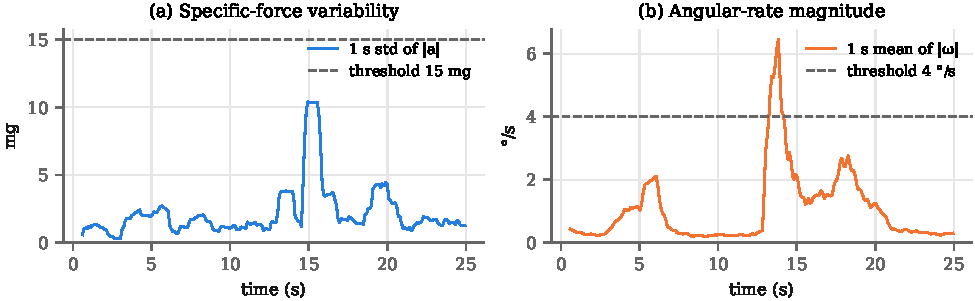
\includegraphics[width=\textwidth]{zupt_detector.pdf}
\caption{ZUPT detector statistics on the bench log with the bridge's thresholds
(dashed). Stationary requires both curves below their thresholds.}
\label{fig:zupt}
\end{figure}

\subsection{Inertial dead-reckoning drift}
\label{sec:val-dr}

The specific force was rotated into NED with the logged attitude, gravity removed,
and integrated twice, with the stationary vehicle as ground truth. The experiment is
intentionally simple (no filter, \SI{10}{\hertz}) and shows error growth, not the
autopilot EKF's performance.

\begin{figure}[H]
\centering
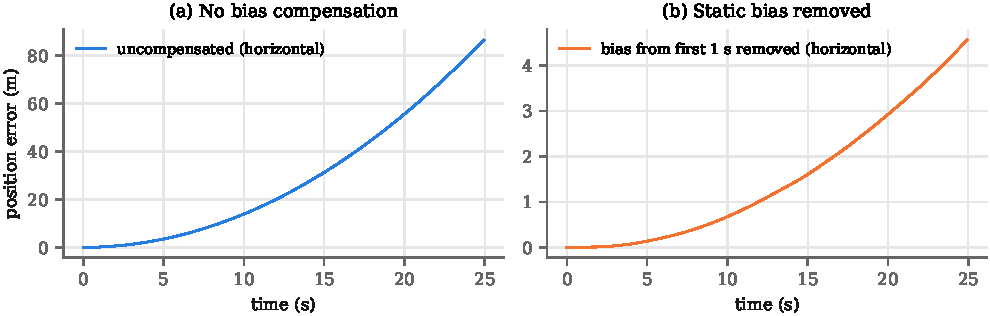
\includegraphics[width=\textwidth]{imu_dead_reckoning.pdf}
\caption{Horizontal position error of strapdown integration on the stationary log.
(a) Uncompensated; (b) after subtracting the mean NED acceleration of the first
second.}
\label{fig:dr}
\end{figure}

\begin{table}[H]
\centering\small
\caption{Horizontal dead-reckoning error on a stationary vehicle.}
\label{tab:dr}
\begin{tabular}{l S[table-format=2.2] S[table-format=2.2] S[table-format=2.2] S[table-format=2.2]}
\toprule
& {$t=\SI{5}{\second}$} & {$t=\SI{10}{\second}$} & {$t=\SI{20}{\second}$} & {$t=\SI{24.9}{\second}$} \\
\midrule
Uncompensated (\si{\metre}) & 3.55 & 14.17 & 56.08 & 86.50 \\
Static bias removed (\si{\metre}) & 0.14 & 0.69 & 2.95 & 4.56 \\
\bottomrule
\end{tabular}
\end{table}

Without compensation, the mean residual horizontal acceleration (north, east) was
$-0.146$ and \SI{0.238}{\metre\per\second\squared}, a magnitude of
\SI{0.279}{\metre\per\second\squared} ($\approx$\SI{28}{\milli\gacc}). \Cref{eq:bias-drift} predicts $\tfrac12(0.279)(24.9)^2=\SI{86.5}{\metre}$, matching
the integrated quadratic error. The residual combines bias, scale error, misalignment
and quantisation, which were not separated. Even after a one-second static bias
calibration the error reached \SI{4.6}{\metre} in \SI{25}{\second}, 90 times the
\SI{5}{\centi\metre} KPI in a 24th of its time window: inertial sensing alone cannot
meet the targets, which is why the design relies on flow, LiDAR and ZUPT.

\subsection{Perception throughput}
\label{sec:val-seg}

\paragraph{Protocol} \code{report/scripts/bench_segmentation.py} instantiates the
project's \code{HybridSegmenter} with the deployed weights
(\code{yolov8n-seg.pt}, \code{sam2.1_t.pt}). It runs 10 warm-up and 100 timed
iterations per configuration on one 640$\times$480 frame, the stream resolution, with
CUDA synchronisation around each call. Host: NVIDIA RTX~4050 Laptop GPU, PyTorch 2.5.1
(CUDA 12.1), Ultralytics 8.4.70, YOLO in FP16. Input: Ultralytics' \code{bus.jpg} at 640$\times$480 (four
instances, all refined by SAM).

\begin{table}[H]
\centering\small
\caption{Per-frame latency of the hybrid segmenter (100 frames each).}
\label{tab:seg}
\begin{tabular}{l S[table-format=2.1] S[table-format=2.1] S[table-format=2.1] S[table-format=1.2] S[table-format=2.1] S[table-format=2.1] S[table-format=3.0]}
\toprule
\textbf{Configuration} & {\textbf{Mean}} & {\textbf{Median}} & {\textbf{p95}} & {\textbf{SD}} & {\textbf{YOLO}} & {\textbf{SAM}} & {\textbf{FPS}} \\
 & {(ms)} & {(ms)} & {(ms)} & {(ms)} & {(ms)} & {(ms)} & \\
\midrule
YOLO only & 5.6 & 5.4 & 6.6 & 0.58 & 4.1 & {--} & 179 \\
YOLO + SAM~2.1-t @\SI{768}{px} & 31.6 & 31.5 & 33.3 & 0.73 & 4.3 & 25.4 & 32 \\
YOLO + SAM~2.1-t @\SI{1024}{px} & 51.4 & 51.3 & 52.8 & 0.81 & 4.5 & 44.8 & 19 \\
\bottomrule
\end{tabular}
\end{table}

\begin{figure}[H]
\centering
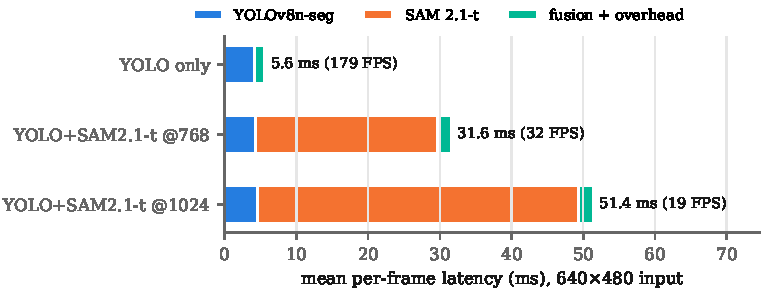
\includegraphics[width=0.78\textwidth]{seg_benchmark.pdf}
\caption{Latency breakdown of the hybrid segmenter on the RTX~4050 Laptop GPU.}
\label{fig:segbench}
\end{figure}

\paragraph{Findings} SAM takes 80--87\% of the frame time. At \SI{768}{px} instead
of \SI{1024}{px} total latency drops 39\% to \SI{31.6}{\milli\second} (32\,FPS), double
the vehicle's \SI{15}{\hertz} camera, so perception is not the bottleneck. This agrees
with our earlier drone-feed measurements (\SI{36}{\milli\second} and
\SI{50}{\milli\second}). Run-to-run SD was below \SI{1}{\milli\second}.

\paragraph{Qualitative output} \Cref{fig:seg} shows hybrid segmentation of a laboratory
scene captured through the vehicle's camera stream. A partly visible object at the left edge is
wrongly labelled \emph{car} (0.45), and the chairs have only moderate confidence
(0.40--0.74). With the camera obstructed (c) the pipeline correctly returns nothing,
illustrating the visual channel's dependence on a clear view.

\begin{figure}[H]
\centering
\begin{subfigure}[t]{0.32\textwidth}
  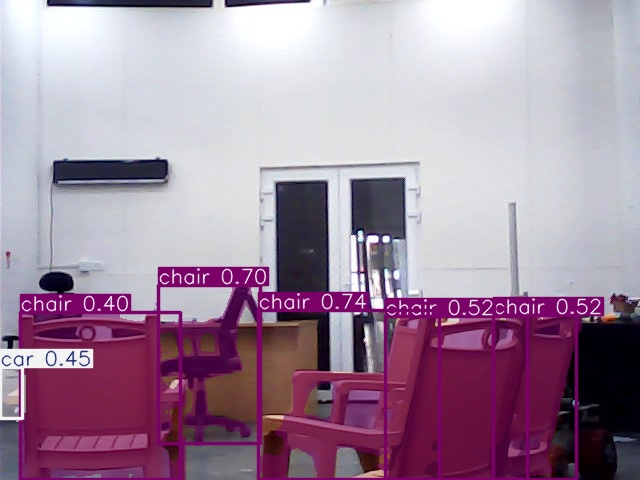
\includegraphics[width=\linewidth]{segmented_result.jpg}
  \caption{Annotated detections.}
\end{subfigure}\hfill
\begin{subfigure}[t]{0.32\textwidth}
  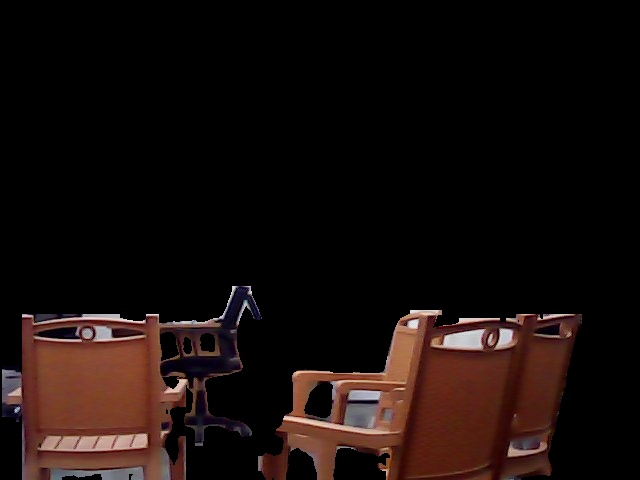
\includegraphics[width=\linewidth]{mask_overlay.jpg}
  \caption{Foreground masks only.}
\end{subfigure}\hfill
\begin{subfigure}[t]{0.32\textwidth}
  
\includegraphics[width=\linewidth]{received_raw_matrix.jpg}
  \caption{Obstructed camera frame.}
\end{subfigure}
\caption{Perception outputs saved by our stand-alone tools
(\code{live_segmentation.py --verify}, \code{camera_receiver.py}) from the vehicle's
camera stream (640$\times$480).}
\label{fig:seg}
\end{figure}

\subsection{Communication link}
\label{sec:val-link}

\Cref{tab:latency} gives our before/after latencies for the changes in
\cref{sec:design-link}. They were measured on one machine, so they isolate software
and queueing delay and exclude Wi-Fi air time; over-the-air latency is not yet
recorded, though the metrics of \cref{eq:latency} are in place.

\begin{table}[H]
\centering\small
\caption{Software-path latency before and after optimisation (project measurement,
single host; Wi-Fi time excluded).}
\label{tab:latency}
\begin{tabularx}{\textwidth}{l l l L}
\toprule
\textbf{Path} & \textbf{Before} & \textbf{After} & \textbf{Main change} \\
\midrule
Pixhawk $\rightarrow$ telemetry sent & \SI{28}{\milli\second} (up to 100) & \SI{5}{\milli\second} & 30\,Hz message intervals, event-driven send \\
Telemetry $\rightarrow$ \topic{/odom} & \SI{20}{\milli\second} @ 10\,Hz & \SI{2}{\milli\second} @ 30\,Hz & publish on arrival, drain backlog \\
\topic{/cmd_vel} $\rightarrow$ Pixhawk & \SI{54}{\milli\second} (up to 100) & \SI{1.4}{\milli\second} & forward on arrival, wake listener \\
\bottomrule
\end{tabularx}
\end{table}

\begin{figure}[H]
\centering
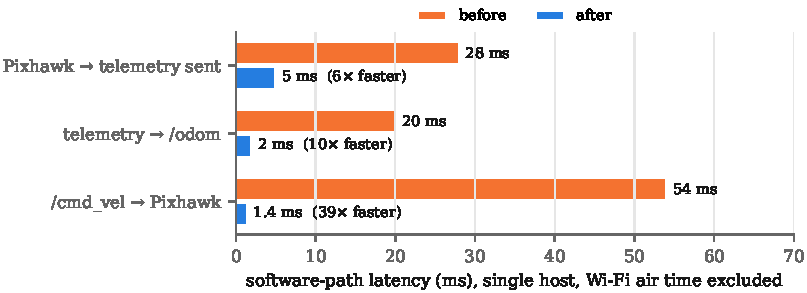
\includegraphics[width=0.78\textwidth]{link_latency.pdf}
\caption{Software-path latency before and after the link optimisations
(\cref{tab:latency}); the command path is 39 times faster.}
\label{fig:latency}
\end{figure}

Nominal rates on the vehicle are \topic{/odom} $\approx$\SI{30}{\hertz},
\topic{/scan} $\approx$\SI{7}{\hertz} (6.4\,rev/s) and camera $\approx$\SI{15}{\hertz}.
Sleeping to enforce the telemetry rate cap delayed fresh bursts by
\SI{15}{\milli\second} (median), so the streamer now skips early sends instead
(\cref{fig:flow-telemetry}). By \cref{eq:frag}, at 5\% fragment loss the
single-datagram LiDAR encoding is delivered with probability 0.95, against 0.86 for the
three-fragment JSON scan.

\subsection{Real-vehicle flight tests}
\label{sec:val-hwdemo}

\paragraph{Hover drift} The vehicle held position in \code{GUIDED} mode, with no GNSS,
for \SI{7}{\minute} at \SI{2.5}{\metre} above a grass surface, using the optical-flow
and rangefinder reference. Drift was measured against marks on the ground with a tape
and the flight video. The total
horizontal drift was \SI{1.6}{\metre}, i.e.\ about \SI{0.23}{\metre\per\minute}.
This is roughly ten times better than the $\ge$\SI{2}{\metre\per\minute} typical of
GNSS-free fallback (\cref{tab:kpi}) and bounded, unlike the inertial-only solution
(\SI{86.5}{\metre} in \SI{25}{\second}, \cref{sec:val-dr}). It is still over 30
times the \SI{5}{\centi\metre}/\SI{10}{\minute} KPI, even over a shorter window. A single run with tape-and-video
ground truth gives the order of magnitude, not a statistical figure.
\Cref{fig:driftcmp} places the hover result beside the inertial-only drift measured on
the same autopilot.

\begin{figure}[H]
\centering
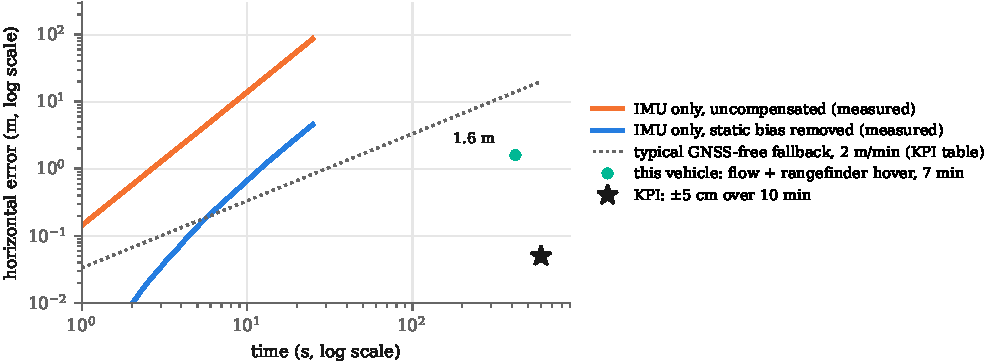
\includegraphics[width=0.92\textwidth]{drift_comparison.pdf}
\caption{Horizontal position error against time (log--log). Inertial-only curves are
from the stationary bench log (\cref{sec:val-dr}); the green point is the
\SI{7}{\minute} flow-and-rangefinder hover at \SI{2.5}{\metre} over grass (only the end
point was measured). The dotted line is the typical GNSS-free fallback and the star the
hover-drift KPI.}
\label{fig:driftcmp}
\end{figure}

\paragraph{Autonomous square path with obstacle avoidance} In a second flight, recorded
outdoors at night (\url{https://youtu.be/y1GYuHiDs4U}, \cref{fig:hwdemo}), Nav2 flew
the vehicle autonomously in \code{GUIDED} mode around a square path among trees, with
the pilot only taking off, landing and standing by. LiDAR returns from trunks and
foliage appear as lethal cells with an inflation layer in the live costmap, and the
planner routed the vehicle around them. The flight shows the complete closed loop on
hardware: sensing on the Pi, the Wi-Fi link, odometry, costmaps, planning and gated
velocity commands back to the autopilot, without ambient light. The video has no
external position reference, so path-following error and avoidance success rate are
not quantified.

\begin{figure}[H]
\centering
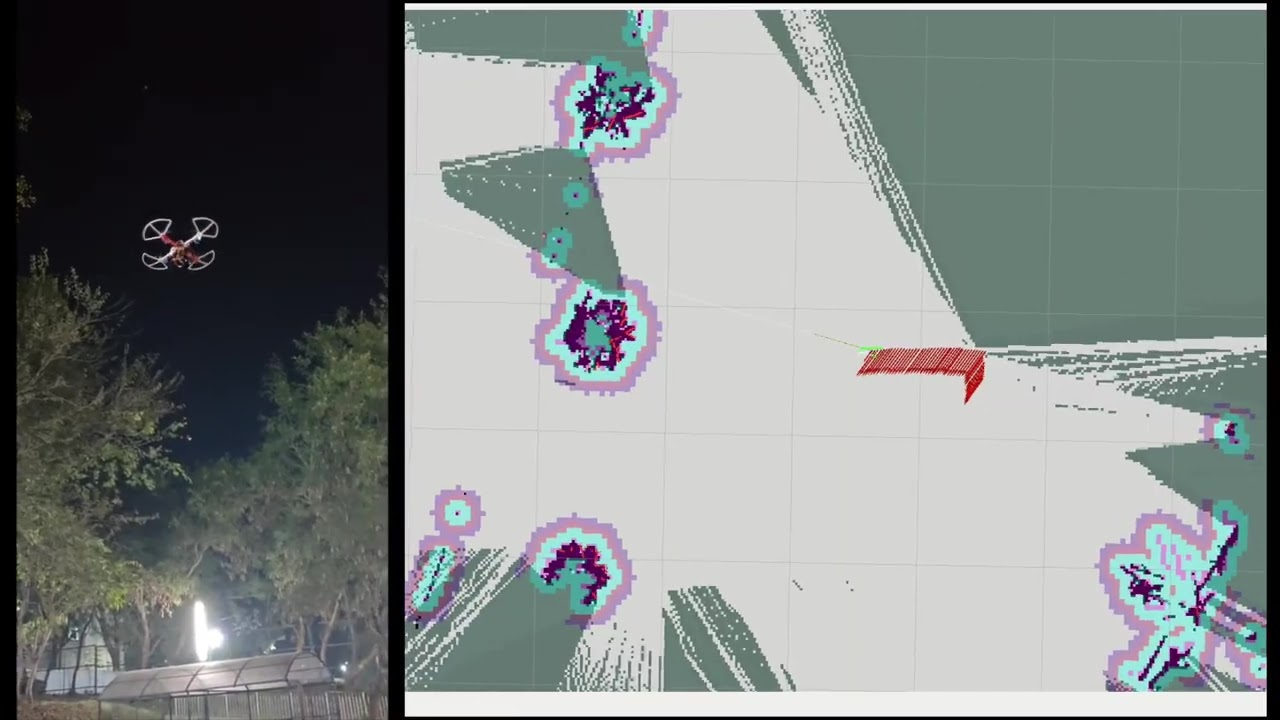
\includegraphics[width=\textwidth]{hardware_demo.jpg}
\caption{Autonomous square-path flight with obstacle avoidance (outdoors, at
night). Left: the quadcopter in flight. Right: live RViz view on the ground computer with LiDAR-derived obstacles
(trees) and their inflated Nav2 costmap, and the vehicle's estimated pose (red). Frame
from the video at \url{https://youtu.be/y1GYuHiDs4U}.}
\label{fig:hwdemo}
\end{figure}

\subsection{Simulation}

In the office world the vehicle explores autonomously until no frontier remains,
then returns to the start. \Cref{fig:sim} shows a frame of a recorded run
(\code{sim_office.launch.py}, video at \url{https://youtu.be/bwV-gUs8EIc}): mapped
free space is confined to rooms already observed, showing frontier-driven coverage.

\begin{figure}[H]
\centering
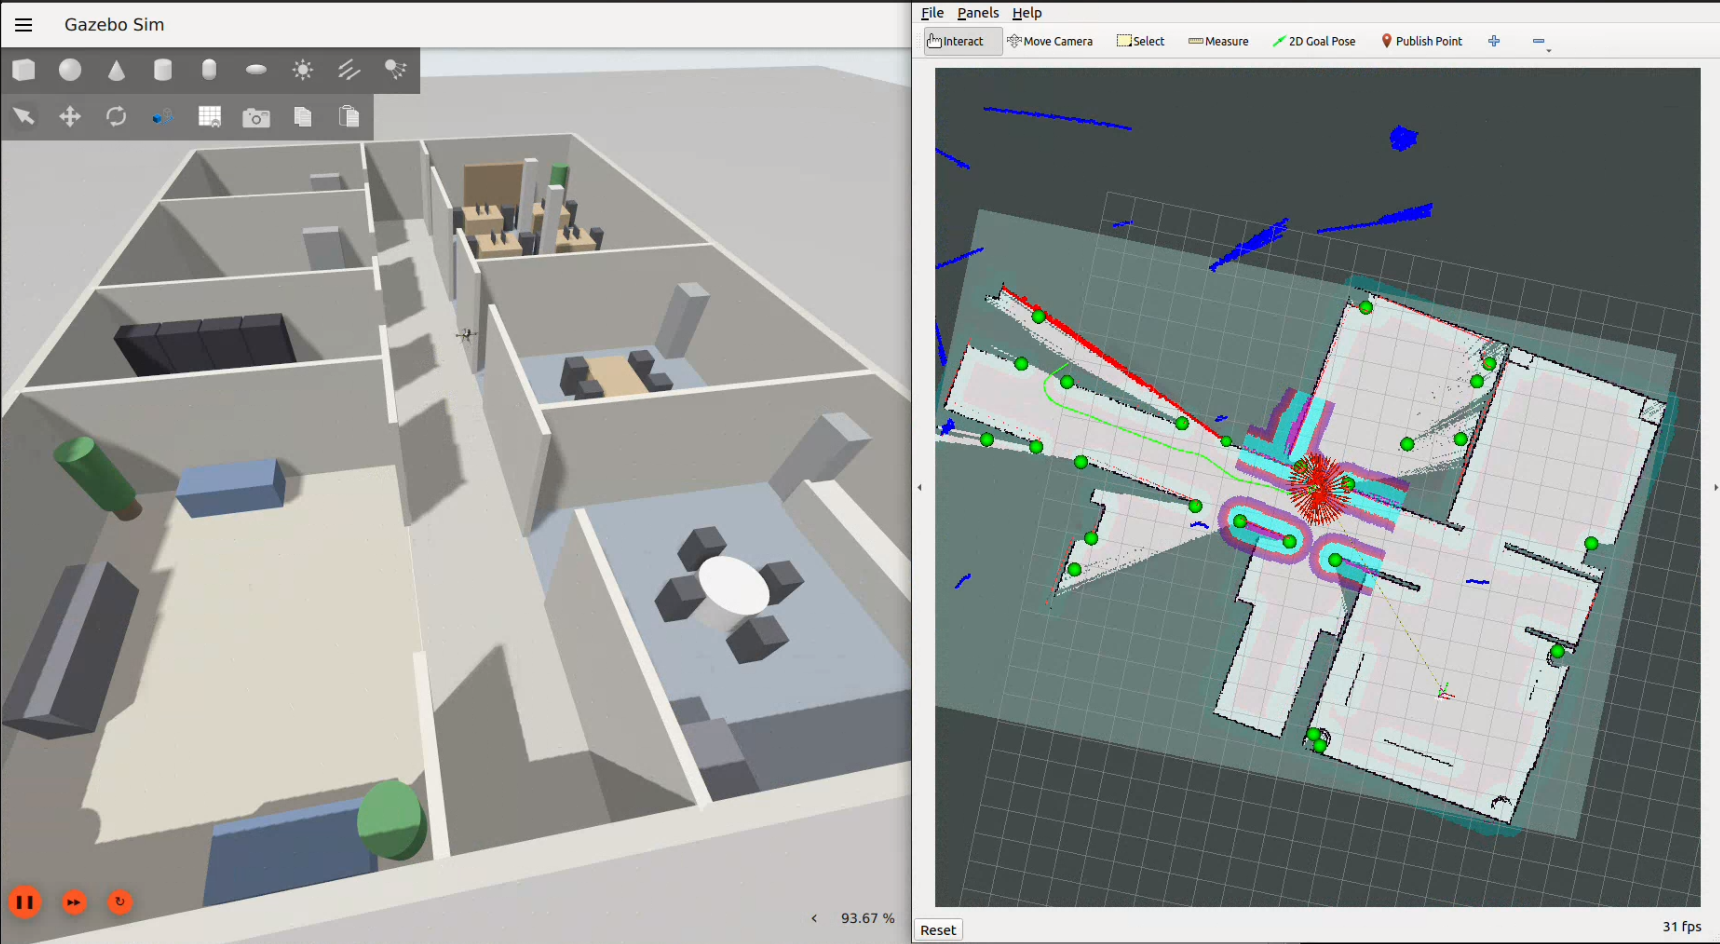
\includegraphics[width=\textwidth]{sim.png}
\caption{Autonomous exploration in the simulated office world (PX4 SITL, Gazebo
Harmonic, ROS~2). Left: Gazebo scene with the x500 in the corridor. Right: RViz with the
SLAM map, inflated costmaps, LiDAR scan, frontier markers (green) and planned path.
Video of the full run: \url{https://youtu.be/bwV-gUs8EIc}.}
\label{fig:sim}
\end{figure}

Simulation also shaped the design: the custom behaviour tree, the projection-based
safety filter (\cref{sec:design-safety}) and a single-instance guard against
\code{TF_OLD_DATA} floods all came from failures observed here.

\subsection{Quantitative analysis of the simulation flight logs}
\label{sec:val-simlogs}

\paragraph{Data} A development session on 20 November 2026 left 34 PX4 ULog files;
26 contain at least \SI{30}{s} armed in \code{OFFBOARD}, totalling \SI{6213}{s}
(\SI{1.7}{h}): 9 office and 17 Baylands flights (six from the open-field spawn).
\code{report/scripts/extract_sim_logs.py} extracts Gazebo ground truth, the EKF2
estimate, the velocity setpoints, the LiDAR scan as PX4 sees it (72 sectors of
\ang{5}) and the flight mode, resampled to \SI{5}{Hz}; \code{make_sim_figures.py}
computes every number below. \code{explore_lite} logs give each exploration's start,
end and termination reason.

Statistics run from \SI{15}{s} after \code{OFFBOARD} starts (excluding take-off) to its
end, or to \SI{2}{s} before the first \emph{fall} (dropping below \SI{0.5}{m} while
commanded higher). Caveats: the software changed between runs; EKF2 fused simulated GPS
in all runs (\code{EKF2_GPS_CTRL}${}=7$), so estimator errors are GPS-aided; and
Gazebo's sensors are idealised.

\paragraph{Sensor model check} To check the data path and frame conventions, every
LiDAR return of one complete exploration was projected at the ground-truth pose into
\SI{10}{cm} cells (\cref{fig:simmap}a). 78\% of cells hit 20 or more times lie within
\SI{0.15}{m} of an object reaching the scan plane; furniture below the plane leaves no
returns, as designed (\cref{sec:op-sim}).

\begin{figure}[p]
\centering
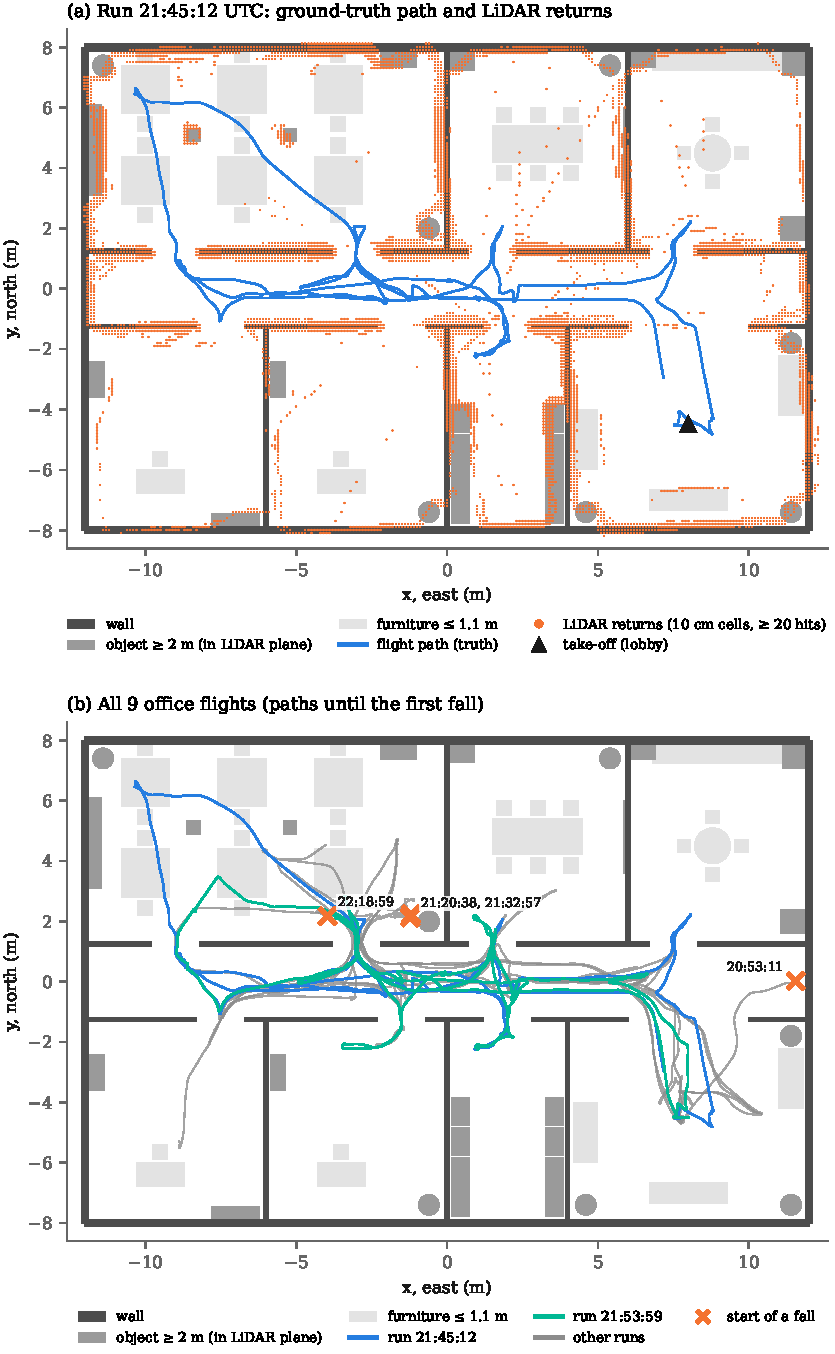
\includegraphics[width=0.84\textwidth]{sim_office_map.pdf}
\caption{Office world, top view (from \code{office.sdf}).
(a)~Run 21:45:12~UTC, a complete autonomous exploration: ground-truth flight path
and the LiDAR returns accumulated at the ground-truth pose.
(b)~All nine office flights, with each path shown until its first fall; crosses mark
where a fall began (\cref{tab:simincidents}).}
\label{fig:simmap}
\end{figure}

\paragraph{Exploration} Three of the office flights ended with \code{explore_lite}
reporting that all frontiers had been traversed or tried, after which the vehicle
returned towards the lobby:
\begin{itemize}[nosep]
  \item 21:45:12 explored for \SI{414}{s} and flew \SI{105.5}{m} with no fall;
  \item 21:53:59 explored for \SI{488}{s} and flew \SI{98.6}{m} with no fall;
  \item 21:32:57 explored for \SI{480}{s}; it fell once, climbed back and carried on.
\end{itemize}
Run 21:45:12 (\cref{fig:simmap}a, \cref{fig:simts}) visited every room except
office~A, which it mapped through the doorway. \Cref{tab:simruns} lists all office
flights and the Baylands flights longer than \SI{10}{m}.

\begin{table}[t]
\centering\footnotesize
\setlength{\tabcolsep}{3.2pt}
\caption{Simulation flights (PX4 SITL + Gazebo; truth from Gazebo). Height: error of
the height above the floor against the commanded height. Speed: horizontal, truth.
Track: RMS of commanded minus estimated velocity. Clear.: nearest LiDAR return.
$<$0.65: share of time inside the bridge's stop distance. Est.: EKF2 horizontal error,
\textbf{GPS-aided}. Baylands*: open-field spawn.}
\label{tab:simruns}
% generated by report/scripts/make_sim_figures.py from sim_runs.csv - do not edit
\begin{tabular}{@{}l l r r r r r r r r r r l@{}}
\toprule
& & \multicolumn{1}{c}{\textbf{OFFB.}} & \multicolumn{1}{c}{\textbf{Path}} &
\multicolumn{2}{c}{\textbf{Height (cm)}} & \multicolumn{2}{c}{\textbf{Speed (m/s)}} &
\multicolumn{1}{c}{\textbf{Track}} & \multicolumn{1}{c}{\textbf{Clear.}} &
\multicolumn{1}{c}{\textbf{$<$0.65}} & \multicolumn{1}{c}{\textbf{Est.}} & \\
\cmidrule(lr){5-6}\cmidrule(lr){7-8}
\textbf{Run (UTC)} & \textbf{World} & (s) & (m) & RMS & max & mean & p95 & (m/s) &
min (m) & (\%) & (cm) & \textbf{Outcome} \\
\midrule
19:09:55 & Baylands* & 182 & 13.5 & 6 & 21 & 0.08 & 0.91 & 0.07 & 16.54 & 0.0 & 4.3 & goals by operator \\
19:19:41 & Baylands* & 235 & 53.0 & 8 & 12 & 0.23 & 0.93 & 0.14 & 0.86 & 0.0 & 7.0 & goals by operator \\
19:28:09 & Baylands* & 429 & 194.0 & 4 & 24 & 0.47 & 0.94 & 0.20 & 0.71 & 0.0 & 18.4 & goals by operator \\
19:49:03 & Baylands & 225 & 43.3 & 6 & 14 & 0.20 & 0.94 & 0.17 & 1.70 & 0.0 & 6.6 & goals by operator \\
20:16:15 & Baylands & 52 & 18.5 & 4 & 17 & 0.46 & 0.99 & 0.49 & 0.39 & 5.9 & 7.8 & goals by operator \\
20:20:36 & Baylands & 533 & 97.5 & 6 & 32 & 0.19 & 0.92 & 0.14 & 0.81 & 0.0 & 5.5 & goals by operator \\
20:49:32 & Office & 137 & 19.9 & 3 & 6 & 0.16 & 0.51 & 0.07 & 0.53 & 13.3 & 4.0 & goals by operator \\
20:53:11 & Office & 370 & 8.6 & 5 & 9 & 0.04 & 0.44 & 0.03 & 0.62 & 0.2 & 3.9 & fall at 230\,s \\
21:00:33 & Office & 196 & 34.0 & 3 & 8 & 0.18 & 0.50 & 0.07 & 0.44 & 12.4 & 5.4 & goals by operator \\
21:04:15 & Baylands & 53 & 31.6 & 4 & 9 & 0.81 & 0.98 & 0.49 & 0.96 & 0.0 & 7.6 & goals by operator \\
21:20:38 & Office & 622 & 64.2 & 4 & 8 & 0.37 & 0.52 & 0.24 & 0.43 & 28.9 & 5.5 & exploring, stopped; fall at 185\,s \\
21:32:57 & Office & 686 & 77.4 & 3 & 20 & 0.30 & 0.51 & 0.23 & 0.59 & 2.3 & 5.3 & explored, all frontiers; fall at 266\,s \\
21:45:12 & Office & 465 & 105.5 & 11 & 47 & 0.23 & 0.51 & 0.13 & 0.62 & 0.4 & 4.6 & explored, all frontiers \\
21:53:59 & Office & 528 & 98.6 & 10 & 45 & 0.19 & 0.50 & 0.12 & 0.62 & 0.1 & 4.1 & explored, all frontiers \\
22:05:42 & Office & 232 & 60.3 & 12 & 42 & 0.27 & 0.52 & 0.15 & 0.66 & 0.0 & 6.5 & exploring, stopped \\
22:18:59 & Office & 118 & 28.0 & 14 & 34 & 0.28 & 0.49 & 0.18 & 0.61 & 2.4 & 3.4 & explored, no frontiers; fall at 108\,s \\
\bottomrule
\end{tabular}

\end{table}

\begin{figure}[t]
\centering
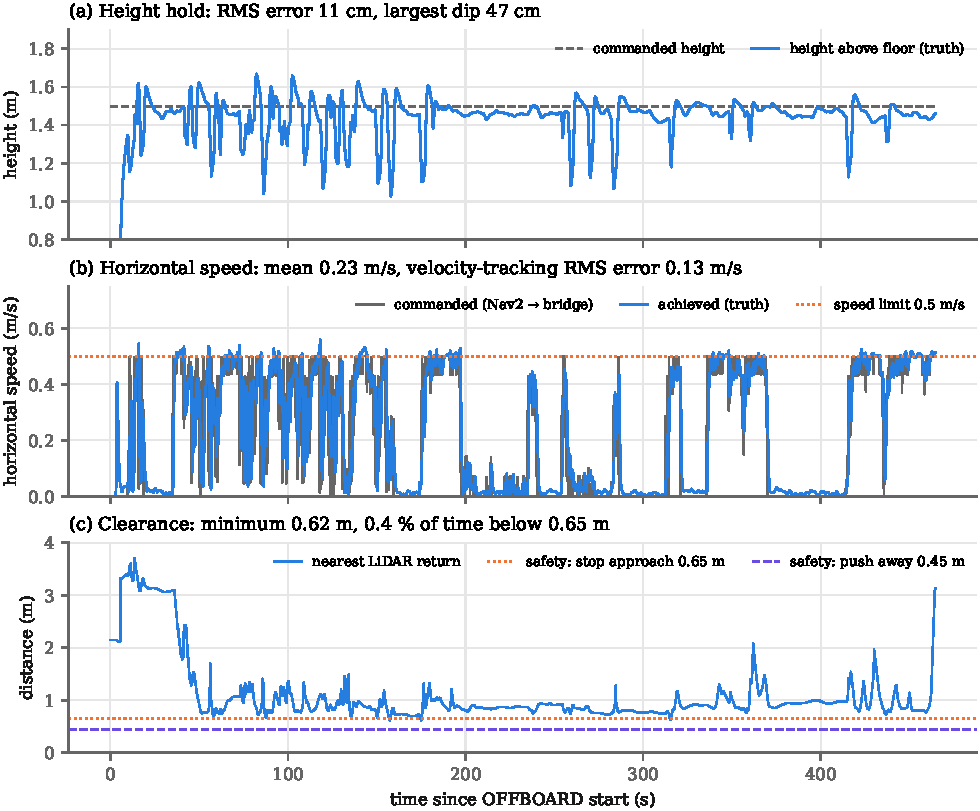
\includegraphics[width=\textwidth]{sim_office_timeseries.pdf}
\caption{Complete office exploration, run 21:45:12~UTC: (a) height above the floor
against the \SI{1.5}{m} command; (b) commanded and achieved horizontal speed against
the \SI{0.5}{m/s} limit; (c) nearest LiDAR return against the bridge's two safety
distances.}
\label{fig:simts}
\end{figure}

\paragraph{Speed and command tracking} Commanded speed never exceeded the configured
limits (\SI{0.5}{m/s} office, \SI{1.0}{m/s} Baylands); the true 95th percentile was at
most \SI{0.52}{m/s} and \SI{0.99}{m/s}. Velocity tracking error was 0.12--\SI{0.24}{m/s}
RMS, mostly at abrupt goal changes (\cref{fig:simts}b). Speed is bimodal
(\cref{fig:simclear}b): hovering while planning, and cruising at the limit.

\paragraph{Height hold} RMS height error was 3--\SI{14}{cm}. Later flights (21:45
onwards) dip up to \SI{47}{cm} when braking, recovering in about \SI{3}{s}
(\cref{fig:simts}a). These dips are a real risk: the office has no furniture between \SI{1.1}{m} and
\SI{2.0}{m}, where the LiDAR plane sits (\cref{sec:op-sim}), and a dip takes the vehicle
into the band of unseen low furniture, as in the 22:18:59 fall.

\paragraph{Clearance} In the two clean explorations the nearest return never fell
below \SI{0.62}{m}; it was inside the \SI{0.65}{m} stop distance 0.4\% and 0.1\% of the
time and never inside \SI{0.45}{m} (\cref{fig:simclear}a). Earlier flights spent
12--13\% (and 21:20:38, before its fall, 29\%) inside \SI{0.65}{m}, e.g.\ at doorways.

\begin{figure}[t]
\centering
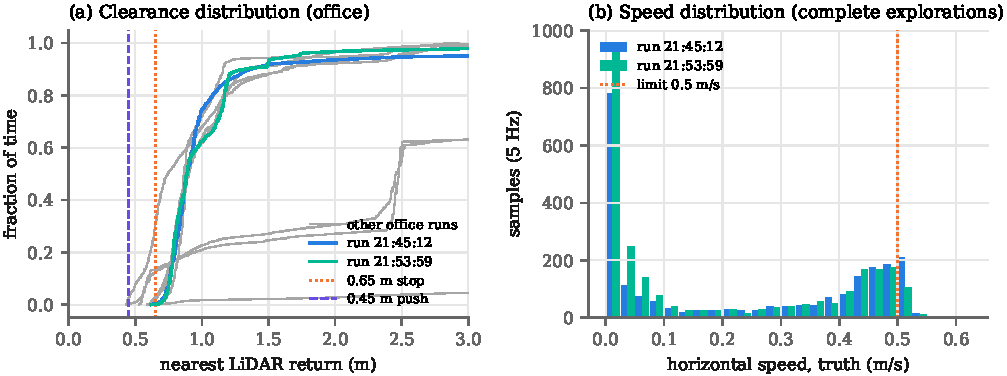
\includegraphics[width=\textwidth]{sim_clearance_speed.pdf}
\caption{(a) Cumulative distribution of the nearest LiDAR return over all office
flights, each up to its first fall. (b) Horizontal speed distribution of the two
complete explorations without a fall.}
\label{fig:simclear}
\end{figure}

\paragraph{Falls} Four office flights contain a fall (\cref{tab:simincidents},
crosses in \cref{fig:simmap}b), each 0.11--\SI{0.31}{m} from the nearest object, well
inside the x500's \SI{0.38}{m} propeller radius, so propeller contact is the likely
cause. The objects were the corridor end wall (20:53:11), the same potted plant at the
open-plan doorway (21:20:38, 21:32:57; later explorations passed it cleanly), and a
\SI{0.95}{m} chair below the LiDAR plane, reached after the vehicle sagged from
\SI{1.6}{m} to \SI{0.9}{m} (22:18:59). At the end wall the nearest return was
\SI{0.62}{m}, more than the true distance, for reasons the logs do not show. The vehicle
recovered height after every fall, and 21:32:57 went on to complete its exploration. One
Baylands log (20:16:15) ends \SI{0.2}{s} after a sudden \SI{5}{m/s} movement; a
collision is possible but unconfirmed and not counted.

\begin{table}[t]
\centering\footnotesize
\caption{Falls in the office flights. Time: since \code{OFFBOARD} start, when the height
began to drop. Position: Gazebo $x$ (east), $y$ (north). Distance: from the vehicle's
centre to the nearest object of \code{office.sdf}. LiDAR: nearest return in the 3\,s
before.}
\label{tab:simincidents}
% generated by report/scripts/make_sim_figures.py from sim_runs.csv - do not edit
\begin{tabular}{@{}l r l l r r l@{}}
\toprule
\textbf{Run (UTC)} & \textbf{Time (s)} & \textbf{Position (m)} & \textbf{Nearest object} &
\textbf{Dist.\ (m)} & \textbf{LiDAR (m)} & \textbf{Afterwards} \\
\midrule
20:53:11 & 230.4 & (11.56, 0.02) & wall, top 3.00\,m & 0.31 & 0.62 & climbed back; goals by operator \\
21:20:38 & 184.8 & (-1.22, 2.13) & plant, top 2.00\,m & 0.28 & 0.19 & climbed back; stopped by operator \\
21:32:57 & 266.1 & (-1.19, 2.23) & plant, top 2.00\,m & 0.28 & 0.42 & climbed back; exploration completed \\
22:18:59 & 107.7 & (-3.96, 2.17) & chair, top 0.95\,m & 0.11 & 0.72 & climbed back; no frontiers left \\
\bottomrule
\end{tabular}

\end{table}

\paragraph{Baylands} \Cref{fig:simbay}a shows the longest Baylands flight with goals
from the operator (\SI{533}{s} in \code{OFFBOARD}, \SI{97.5}{m}). The tree crowns appear
as clusters of LiDAR returns in the scan plane. The flight passes between them with a
minimum clearance of \SI{0.81}{m}.

Over all flights longer than \SI{5}{m}, EKF2's horizontal RMS error against ground
truth is at most \SI{18}{cm} (maximum \SI{36}{cm}; \cref{fig:simbay}b). Being
GPS-aided, this shows only that Nav2 received a consistent pose.

\begin{figure}[t]
\centering
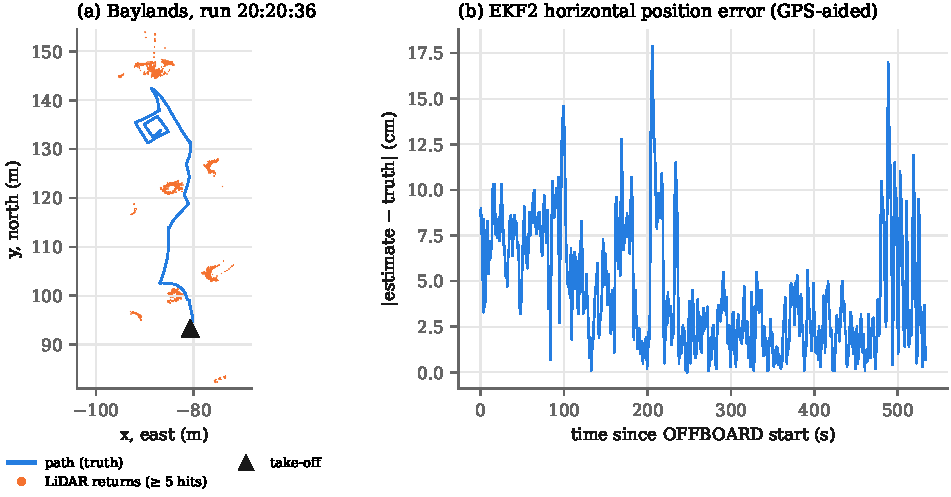
\includegraphics[width=\textwidth]{sim_baylands.pdf}
\caption{Baylands, run 20:20:36~UTC: (a) ground-truth path and accumulated LiDAR
returns (tree crowns in the scan plane); (b) horizontal error of EKF2's position
estimate against Gazebo truth, with simulated GPS fused.}
\label{fig:simbay}
\end{figure}
